\chapter{战术导弹动力学建模以及动力学特性分析}
\section{导弹动力学传递函数}
\section{导弹动力学8个特点}
\begin{enumerate}[1)]
    \item 直联项的影响
    \item 静稳定度$a_{24}$越大,固有频率越高
    \item 静稳定度越大,阻尼$\xi$越小
    \item 导弹极点并不会随着静稳定度变大而向左移,而是沿着平行于虚轴的直线远离实轴
    \item 静稳定度越大,导弹的响应速度越快。
    
    {\kaishu 此处注意区分理解“快速性”和“操纵性”:操纵性是导弹产生法向过载的难易程度,
    而阶跃响应的时间$t_r = \frac{\pi - arccos\xi_{\dot{m}}}{\omega_{m}\sqrt{1-\xi_{m}^2}}$
    可以描述导弹的“快速性”
    
    补充:《自动控制原理》
    
    一个欠阻尼二阶系统,其两个极点的复域如图\ref{exrem_point}所示:
    \begin{figure}[H]
        \centering
        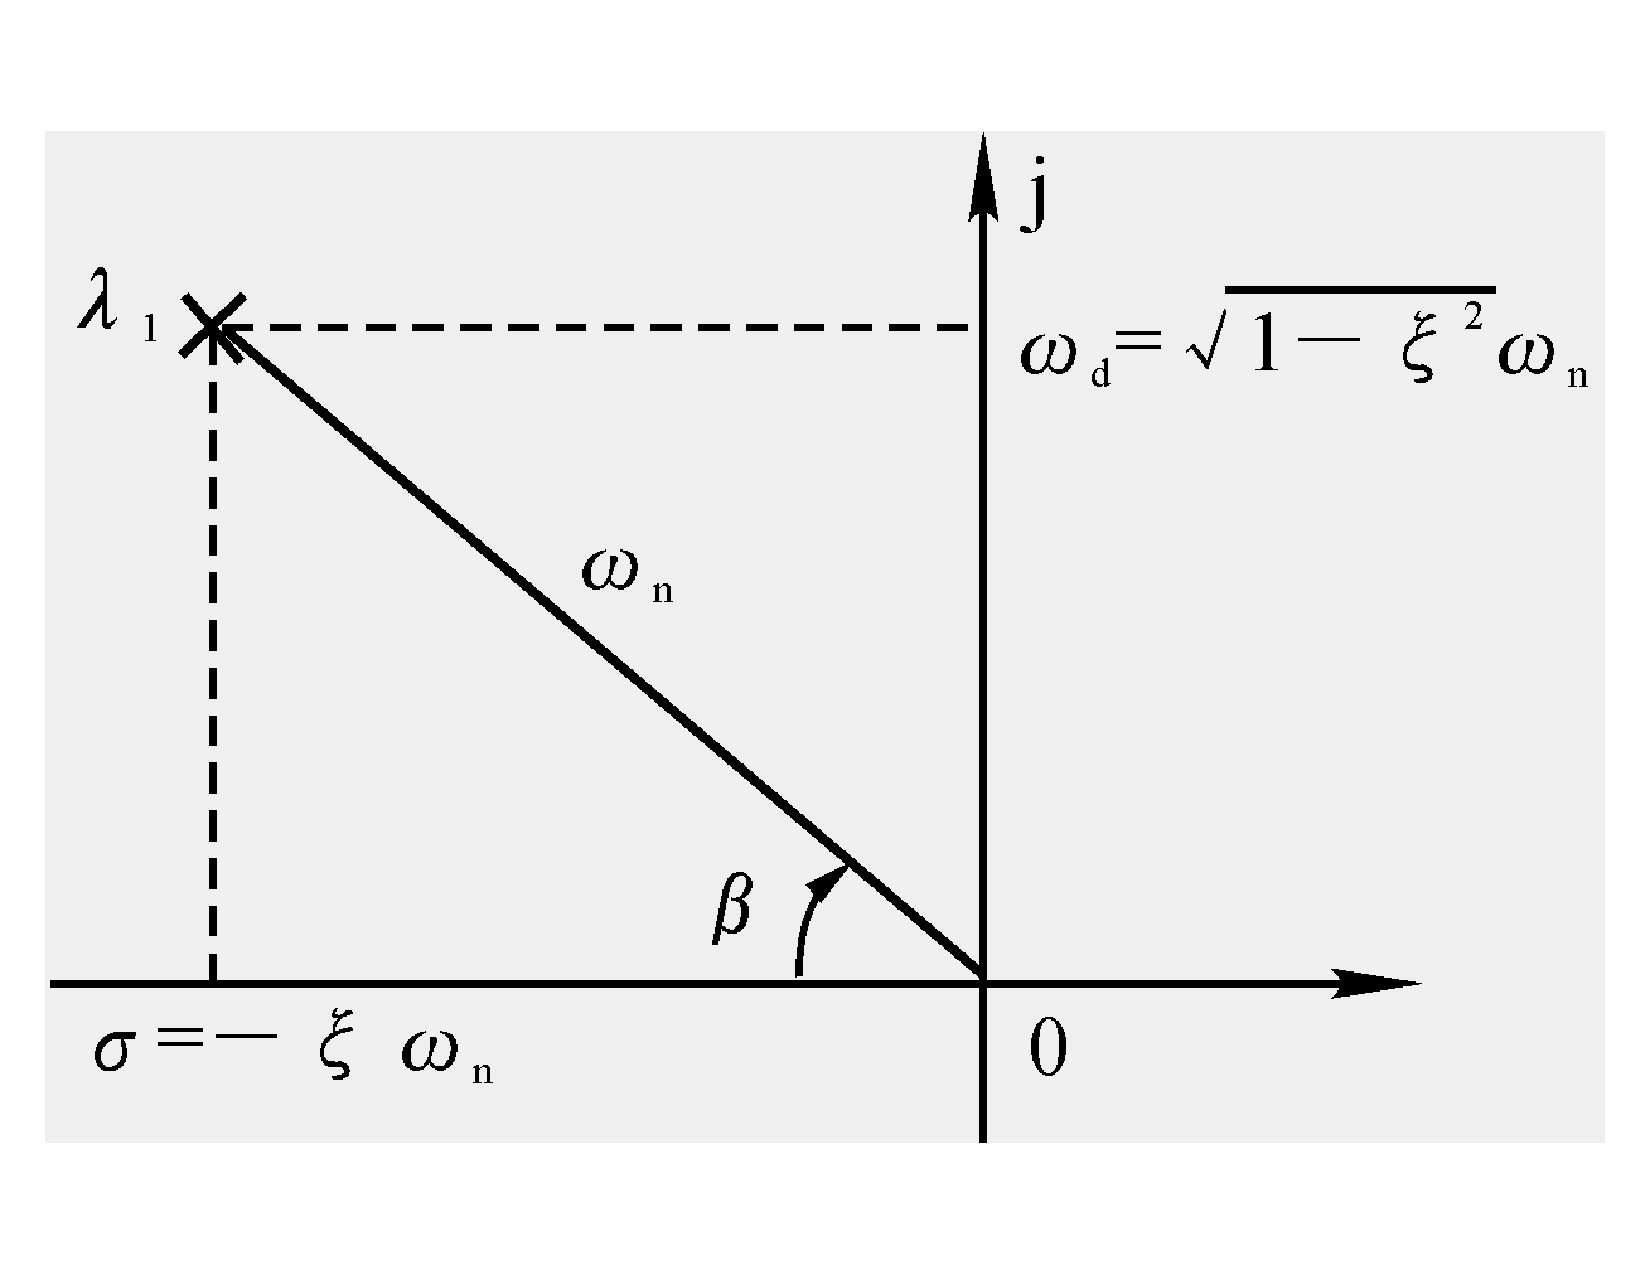
\includegraphics[scale = 0.35]{pictures/2_order}
        \caption{二阶欠阻尼系统极点}
        \label{exrem_point}
    \end{figure}
    \begin{enumerate}[i]
        \item 阻尼比:$\xi = \cos\beta$ 
        \item 上升时间:$t_r = \frac{\pi-\beta}{\omega_d}$,其中$\beta = arccos\xi$
        \item 峰值时间:$t_p = \frac{\pi}{\omega_d}$
        \item 最大超调量:$\sigma\% = e^{-\pi\xi\sqrt{1-\xi^2}}\times100\%$
        \item 调节时间:当$\Delta = 0.5$时,$t_s\approx \frac{3}{\xi\omega_n}$;
                        当$\Delta = 0.3$时,$t_s\approx \frac{4}{\xi\omega_n}$;
    \end{enumerate}
    }
    \item 鸭式导弹和正常布局导弹的响应速度并无区别;鸭式导弹的稳态增益大于正常布局导弹,
    在0时刻的导弹的法向加速度,鸭式为正,正常式为负。(其实就是考虑直联项的影响)
    \item 静稳定的导弹考虑只短周期时,两个极点是在左半开平面,但长周期未必都在。
    \item 导弹动力学本身就是一个具有反馈的系统,“过载自动驾驶仪就是弹体动力学的自然延伸。”
\end{enumerate}
\section{状态空间表达式下的弹体动力学}